%!TEX root = ../thesis.tex

\tikzstyle{database} = [cylinder, shape border rotate=90, aspect=0.5, draw, fill=green!30],
\tikzstyle{node} = [rectangle, minimum width=4cm, minimum height=1cm, text centered, draw=black, draw, fill=blue!30],
\tikzstyle{blockchain} = [draw,rectangle,minimum width=\textwidth, minimum height=1cm,anchor=west, fill=orange!30],
\tikzstyle{process} = [fill=red!30],
\tikzstyle{txt} = []

\chapter{Solution}
\label{solution}

In our solution the blockchain is used as the controller of the application. It is responsible for keeping an
audit immutable log of all actions of the participants. All interaction are being made
through the blockchain supporting data accountability and provenance tracking. It should be mention that blockchain does not offers an extra security layer as the data are off-chain and data silos remain a single point of failure.

\section{Trust model}
\label{solution:trust_model}

In our model we assume that the involved entities that interact with a data set--the data controller and the data processor-- are identified and verified through a public key infrastructure (PKI)~\cite{adams_understanding_2003}. Furthermore, each entity is a trusted entity with certain trust properties. In particular, the data controller is trusted for integrity and confidentiality and the data processor only for confidentiality.

\section{Entities}
\label{solution:entities}

There are three main roles consisting the application: the data controller, the data processor
and the data requester. The first two are also defined in the context of GDPR (§~\ref{problem:regulations}).
GDPR defines another role, that of data subject-the owner of the data.
In our scheme we assume that the data controller already has permission to access the data or
she is at the same time the data subject and the data controller.

\subsection{Data Controller}
\label{solution:entities:data_controller}

The data controller is in charge of a data set. She run on behalf of a data subject (person)
that authorizes the data controller to access her personal data, with the possibility of forwarding
them to a data processor that will be responsible for processing the data on behalf of controller~\cite{DBLP:journals/corr/NeisseSF17}.

\subsection{Data Processor}
\label{solution:entities:data_processor}

The data processor is responsible for processing data on behalf of the data requester. She listens
for data processing requests and returns, along with the output of the process, a Zero Knowledge Proof of correct computation over the requested data set.

\subsection{Data Requester}
\label{solution:entities:data_req}

The requester can be any entity that requests a computation over a data set. It can be a research center, a university, a machine learning algorithm or any individual. The requester expects, along with the output, a proof of correct computation over the requested data set that verifies when the result of the processing is available.

\section{Queries}
\label{solution:queries}

The system should support only a set of open pre-fabricated queries that have been analyzed and constructed to be privacy-preserving with the use of techniques such as k-anonymity~\cite{Samarati98protectingprivacy} and l-diversity~\cite{Aggarwal2008}. The queries return only de-identified aggregated results.

The supported queries are:

\begin{enumerate}
  \item Sum
  \item Average
  \item Count
  \item Maximum
  \item Median
  \item Minimum
\end{enumerate}

The above queries are not considered to be privacy-preserving as it is outside the scope of the initial prototype and should be implemented on future work.

\section{Consent}
\label{solution:consent}

Modeling dynamic consent in smart contracts should be carefully analyzed taking into account design issues that are related to smart contracts lifecycle, required state variables for storing contract’s information, and access restrictions to those variables.

Neisse et al.~\cite{DBLP:journals/corr/NeisseSF17} proposed the following three models for data accountability and provenance tracking that comply with the GDPR(§~\ref{problem:regulations}):

\begin{enumerate}
  \item Contract for a specific controller: A contract where the data subject creates a contract tailored for each data controller
  \item Contract for specific data: A contract where each subject’s data instance is shared among all data controllers
  \item Contract for multiple data subjects: A contract where the data controller specifies how the data from all subjects are treated from the controller
\end{enumerate}

The first contract is more adequate for sensitive data~\cite{DBLP:journals/corr/NeisseSF17}, such as health data, since a subject-controller relationship~\cite{Azaria2016} is being created where each patient has a different contract for each controller accessing their data, providing fine grained access control and provenance information. On the other hand, it has the highest cardinality among the others two types~\cite{DBLP:journals/corr/NeisseSF17}. The second contract suffers from direct linkability as a unique subject address is needed compromising patients’ privacy~\cite{DBLP:journals/corr/NeisseSF17}. Lastly, the third one has the lowest cardinality among the others but also has the lower level of customization due to the limited number of contract options~\cite{DBLP:journals/corr/NeisseSF17}.

\section{Flow}
\label{solution:flow}

\subsection{Dataset Registration}
\label{solution:flow:reg_data}

\begin{enumerate}
  \item Encrypts a data set with a symmetric key and save it to a specific location
  \item Registers the data set by initiating a transaction that saves the data set's metadata (name, location, category, digest) on the Blockchain.
\end{enumerate}

\begin{figure}[ht!]
  \begin{tikzpicture}[
        database/.style={
        cylinder,
        shape border rotate=90,
        aspect=0.5,
        draw
      },
      txt/.style={
      }
    ]

    \node[draw,rectangle,minimum width=\textwidth, minimum height=1cm,anchor=west] (blockchain) at (0,0){Blockchain};

    \begin{scope}[node distance=4cm]
      \node[draw, minimum height=1cm, minimum width=4cm, anchor=west] (owner) at (0,-5) {Data Controller};
      \node[database] (db) [below right=of owner] {Datastore};
      \draw[<->] (owner) -- (db);
      \draw[<-] ([xshift=-1em]owner.north) -- ([xshift=-1em]2,-0.5);
      \draw[->] ([xshift=1em]owner.north) -- ([xshift=1em]2,-0.5);
    \end{scope}

    \node[txt] (enc_db) [below=of owner,yshift=0em, xshift=10em] {$Enc_k(data)$};
    \node[txt] (enc_key) [above=of owner, xshift=19em, yshift=1em] {$Tx(\{name, location, category, digest, address, hashMeta\}, "register\_data")$};

  \end{tikzpicture}
  \caption{Data registration}
  \label{fig:arc:reg}
\end{figure}

\subsection{Processor Registration}
\label{solution:flow:pr_reg}

\begin{enumerate}
  \item Generates an asymmetric encryption key pair
  \item Registers availability by initiating a transaction that saves processors name and public key on the blockchain
\end{enumerate}

\begin{figure}[ht!]
  \begin{tikzpicture}[
        database/.style={
        cylinder,
        shape border rotate=90,
        aspect=0.5,
        draw
      },
      txt/.style={
      }
    ]

    \node[draw,rectangle,minimum width=\textwidth, minimum height=1cm,anchor=west] (blockchain) at (0,0){Blockchain};


    \begin{scope}
      \node[draw, minimum height=1cm, minimum width=4cm, anchor=west] (processor) at (0,5) {Data Processor};
      \draw[<-] ([xshift=-1em]processor.south) -- ([xshift=-1em]2,0.5);
      \draw[->] ([xshift=1em]processor.south) -- ([xshift=1em]2,0.5);
    \end{scope}

    \node[txt] (enc_db) [below=of processor,yshift=-1.5em, xshift=14em] {$Tx(\{name, pubKey, address\}, "register\_processor")$};

  \end{tikzpicture}
  \caption{Processor Registration}
  \label{fig:arch:pr_reg}
\end{figure}

\subsection{Request for processing}
\label{solution:flow:pr_reg}

\begin{enumerate}
  \item The requestor selects a data set on which the processing should be made and  notify the network participants of the request by initiating a transaction on the blockchain passing along her public key
  \item The controller, responsible for the desired data set, selects a processor and encrypts the symmetric key with the public key of the selected processor
  \item The controller notifies the processor by initiating a transaction on the blockchain passing all needed information such as the encrypted symmetric key and the request ID.
\end{enumerate}

\begin{figure}[ht!]
  \begin{tikzpicture}[
        database/.style={
        cylinder,
        shape border rotate=90,
        aspect=0.5,
        draw
      },
      txt/.style={
      }
    ]

    \node[draw,rectangle,minimum width=\textwidth, minimum height=1cm,anchor=west] (blockchain) at (0,0){Blockchain};

    \begin{scope}[node distance=4cm]
      \node[draw, minimum height=1cm, minimum width=4cm, anchor=west] (owner) at (0,-5) {Data Controller};
      \draw[->] ([xshift=0em]owner.north) -- ([xshift=0em]2,-0.5);
    \end{scope}

    \node[txt] (enc_key) [above=of owner, xshift=11.2em, yshift=13em] {$Tx(requestID, Enc_{pk_P}(k), "notify\_processor")$};

    \node[txt] (list_req) [below=of owner, xshift=0em, yshift=1.5em] {$listen("request\_processing")$};

    \begin{scope}
      \node[draw, minimum height=1cm, minimum width=4cm, anchor=west] (processor) at (0,5) {Data Processor};
      \draw[<-] ([xshift=0em]processor.south) -- ([xshift=0em]2,0.5);
    \end{scope}

    \node[txt] (list_req_cr) [above=of processor, xshift=0em, yshift=-1.5em] {$listen("processing")$};

    \begin{scope}
      \node[draw, minimum height=1cm, minimum width=4cm, anchor=east] (requester) at (\textwidth,-5) {Requester};
      \draw[->] ([xshift=0em]requester.north) -- ([xshift=0em]14.45,-0.5);
    \end{scope}

    \node[txt] (enc_db) [above left=of requester, xshift=7em, yshift=1em] {\footnotesize $Tx(\{dataSetID, queryID, pubKey, address\}, "request\_processing")$};

  \end{tikzpicture}
  \caption{Request for processing}
  \label{fig:arch:req_pr}
\end{figure}

\subsection{Data set processing}
\label{solution:flow:pr_data}

\begin{enumerate}
  \item Process the data
  \item Encrypts the results with the public key of the requestor
  \item Submits the encrypted result of the computation on the blockchain along with a Zero Knowledge Proof (§~\ref{zkp}) of the correctness of the computation.
\end{enumerate}

\begin{figure}[ht!]
  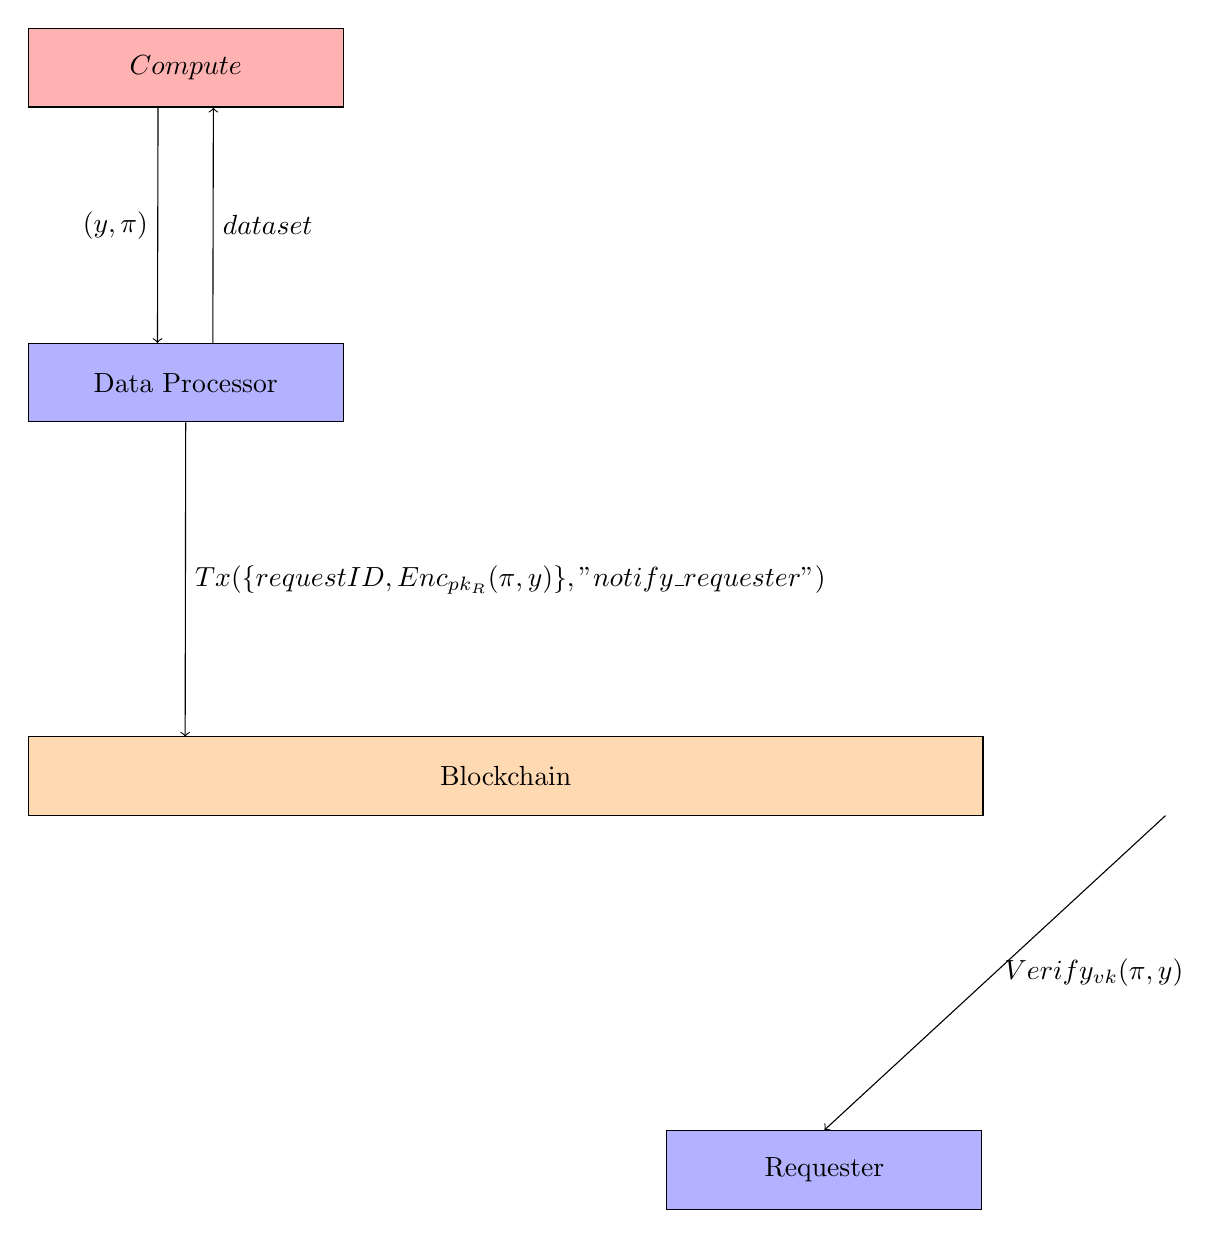
\begin{tikzpicture}

    \node[blockchain] (blockchain) at (0,0){Blockchain};

    \begin{scope}
      \node[node, anchor=west] (processor) at (0,5) {Data Processor};
      \draw[->] ([xshift=0em]processor.south) -- ([xshift=0em]2,0.5) node[midway,right] {$Tx(\{requestID, Enc_{pk_R}(\pi, y)\}, "notify\_requester")$};
    \end{scope}

    \node[node, process] (compute) [above of=processor, yshift=3cm] {$Compute$};

    \draw[->] ([xshift=-1em]compute.south) -- ([xshift=-1em]2,5.5) node[midway,left] {$(y, \pi)$};
    \draw[<-] ([xshift=1em]compute.south) -- ([xshift=1em]2,5.5)  node[midway,right] {$dataset$};

    \begin{scope}
      \node[node, anchor=east] (requester) at (\textwidth,-5) {Requester};
      \draw[<-] (requester.north) -- (14.45,-0.5) node[midway,right] {$Verify_{vk}(\pi, y)$};
    \end{scope}

  \end{tikzpicture}
  \caption{Data processing}
  \label{fig:arch:process}
\end{figure}

\section{Processor Selection}
\label{solution:pr_selection}

\section{Proof of correctness of computation}
\label{solution:proof}

Let $d$ be a private dataset, $H$ a cryptographic hash function and $h = H(d)$ the digest of $d$ over $H$. Let $\calp$ be a prover (data processor) and $\calv$ the verifier (data requester). $\calp$ wants to prove to $\calv$ that

$\calp$ zk-SNARK proof(§~\ref{zkp:snarks}) consists of two parts: a) Knowledge of a pre-image $d$ such that $H(d) = h$ and b) a correct computation over $d$.

\begin{figure}[ht!]
  \begin{tikzpicture}[
        database/.style={
        cylinder,
        shape border rotate=90,
        aspect=0.5,
        draw
      },
      txt/.style={
      }
    ]

    \node[draw,rectangle,minimum width=\textwidth, minimum height=1cm,anchor=west] (blockchain) at (0,0){Blockchain};

    \begin{scope}[node distance=4cm]
      \node[draw, minimum height=1cm, minimum width=4cm, anchor=west] (owner) at (0,-5) {Data Controller};
      \node[database] (db) [below right=of owner] {Database};
      \draw[<->] (owner) -- (db);
      \draw[<-] ([xshift=-1em]owner.north) -- ([xshift=-1em]2,-0.5);
      \draw[->] ([xshift=1em]owner.north) -- ([xshift=1em]2,-0.5);
    \end{scope}

    \node[txt] (enc_db) [below=of owner,yshift=-1.5em, xshift=3em] {$Enc_k(data)$};
    \node[txt] (enc_key) [above=of owner, xshift=6.5em, yshift=1em] {$Enc_{pk_P}(k, metadata)$};

    \begin{scope}
      \node[draw, minimum height=1cm, minimum width=4cm, anchor=west] (processor) at (0,5) {Data Processor};
      \draw[<-] ([xshift=-1em]processor.south) -- ([xshift=-1em]2,0.5);
      \draw[->] ([xshift=1em]processor.south) -- ([xshift=1em]2,0.5);
    \end{scope}

    \node[txt] (enc_db) [below=of processor,yshift=-1.5em, xshift=6em] {$Enc_{pk_R}(result, \pi)$};

    \begin{scope}
      \node[draw, minimum height=1cm, minimum width=4cm, anchor=east] (requester) at (\textwidth,-5) {Requester};
      \draw[->] ([xshift=-1em]requester.north) -- ([xshift=-1em]14.45,-0.5);
      \draw[<-] ([xshift=1em]requester.north) -- ([xshift=1em]14.45,-0.5);
    \end{scope}

    \node[txt] (enc_db) [above left=of requester, xshift=5.5em] {$Request(pk_R, pred)$};
    \node[txt] (enc_db) [above right=of requester, xshift=-5.5em] {$Verify_{vk}(\pi)$};

  \end{tikzpicture}
  \caption{Architecture}
  \label{fig:architecture}
\end{figure}
